\documentclass[]{elsarticle} %review=doublespace preprint=single 5p=2 column
%%% Begin My package additions %%%%%%%%%%%%%%%%%%%
\usepackage[hyphens]{url}

  \journal{An Elsevier journal} % Sets Journal name


\usepackage{lineno} % add
\providecommand{\tightlist}{%
  \setlength{\itemsep}{0pt}\setlength{\parskip}{0pt}}

\usepackage{graphicx}
\usepackage{booktabs} % book-quality tables
%%%%%%%%%%%%%%%% end my additions to header

\usepackage[T1]{fontenc}
\usepackage{lmodern}
\usepackage{amssymb,amsmath}
\usepackage{ifxetex,ifluatex}
\usepackage{fixltx2e} % provides \textsubscript
% use upquote if available, for straight quotes in verbatim environments
\IfFileExists{upquote.sty}{\usepackage{upquote}}{}
\ifnum 0\ifxetex 1\fi\ifluatex 1\fi=0 % if pdftex
  \usepackage[utf8]{inputenc}
\else % if luatex or xelatex
  \usepackage{fontspec}
  \ifxetex
    \usepackage{xltxtra,xunicode}
  \fi
  \defaultfontfeatures{Mapping=tex-text,Scale=MatchLowercase}
  \newcommand{\euro}{€}
\fi
% use microtype if available
\IfFileExists{microtype.sty}{\usepackage{microtype}}{}
\bibliographystyle{elsarticle-harv}
\usepackage{graphicx}
% We will generate all images so they have a width \maxwidth. This means
% that they will get their normal width if they fit onto the page, but
% are scaled down if they would overflow the margins.
\makeatletter
\def\maxwidth{\ifdim\Gin@nat@width>\linewidth\linewidth
\else\Gin@nat@width\fi}
\makeatother
\let\Oldincludegraphics\includegraphics
\renewcommand{\includegraphics}[1]{\Oldincludegraphics[width=\maxwidth]{#1}}
\ifxetex
  \usepackage[setpagesize=false, % page size defined by xetex
              unicode=false, % unicode breaks when used with xetex
              xetex]{hyperref}
\else
  \usepackage[unicode=true]{hyperref}
\fi
\hypersetup{breaklinks=true,
            bookmarks=true,
            pdfauthor={},
            pdftitle={Do Drivers Dream of Walking? An Investigation of Dissonance in the Primary Mode of Travel from the Perspective of Subjective Wellbeing},
            colorlinks=false,
            urlcolor=blue,
            linkcolor=magenta,
            pdfborder={0 0 0}}
\urlstyle{same}  % don't use monospace font for urls

\setcounter{secnumdepth}{0}
% Pandoc toggle for numbering sections (defaults to be off)
\setcounter{secnumdepth}{0}
% Pandoc header
\usepackage{booktabs}
\usepackage{longtable}
\usepackage{array}
\usepackage{multirow}
\usepackage{wrapfig}
\usepackage{float}
\usepackage{colortbl}
\usepackage{pdflscape}
\usepackage{tabu}
\usepackage{threeparttable}
\usepackage{threeparttablex}
\usepackage[normalem]{ulem}
\usepackage{makecell}
\usepackage{xcolor}



\begin{document}
\begin{frontmatter}

  \title{Do Drivers Dream of Walking? An Investigation of Dissonance in the
Primary Mode of Travel from the Perspective of Subjective Wellbeing}
    \author[Some University]{Author 1\corref{c1}}
   \ead{a1@university.com} 
   \cortext[c1]{Corresponding Author}
    \author[Some School]{Author 2}
   \ead{a2@school.com} 
  
      \address[Some University]{Department, Street, City, State, Zip}
    \address[Some School]{Department, Street, City, State, Zip}
  
  \begin{abstract}
  Transportation in most of the world has been dominated for decades by a
  fascination with the automobile. Increasingly, however, it is recognized
  that to achieve a variety of economic, environmental, and public health
  policy goals it is important to attract and retain users of public
  transport and active travel. A challenge with the way transportation
  policy is developed is that it tends to focus on cost-benefit and
  utilitarian considerations, which may miss other potential benefits of
  transportation. For this reason, subjective wellbeing (SWB) has been
  proposed as a way to enhance our understanding of the preferences and
  choices of travellers, as well as a way to evaluate the benefits of
  transportation beyond utilitarian considerations. The objective of this
  paper is to analyze the modes that people commonly use, and to what
  extent they are aligned (or not) with a variety of affective and
  utilitarian values. In other words, we are interested in the potential
  for dissonance with respect to the primary mode of travel, from the
  perspective of affective and utilitarian values. The study is based on
  data collected from a sample of travellers in the city of Santiago, in
  Chile. Participants in the study were asked about their usual mode of
  travel, and then were asked to name the mode or modes that they
  associated to affective values (freedom, enjoyment, and happiness) and
  to utilitarian values (safety, time waste, and efficiency). The results
  indicate that users of public transportation experience the most
  dissonance in terms of affective values, and active travellers the
  least. For those travellers who experience dissonance, active travel is
  the mode most commonly associated with affective values.
  
  To properly assess transportation policy This poses a number of
  challenges Broadening the commonly used transport project assessment
  will be relevant for achieving this goal. While satisfaction with travel
  has been mainly used in the context of daily trips and mainly under
  cost-benefit and utilitarian considerations, subjective wellbeing (SWB)
  over time has risen as an alternative for understanding the preferences
  and choices of transport users. The aim of this paper is to analyse the
  factors that can potentially affect the levels of SWB in the wide
  spectrum of public, private and active transport modes in the context of
  Santiago de Chile. The paper aims to reflect on the possibilities of
  increasing the SWB with a view to enhance the attractiveness of public
  transport and active travel. The paper investigates the affective and
  instrumental/utilitarian factors of SWB, according to modal choice. It
  uses an analysis of correspondence that considers the actual primary
  mode used, versus the mode that each individual associated to both
  utilitarian and affective SWB factors. The results show that there is
  more persistent modal dissonance between positive emotional and
  utilitarian associations within the more disadvantaged groups --
  particularly among users of public transport. The study shows that apart
  from time-savings and efficiency, security has also been
  cross-sectionally sensitive according to the data analysed. Factors such
  as happiness, enjoyment and freedom require far more attention in
  transport planning as they are strongly related to the dimensions of
  subjective and personal wellbeing. Targeting these factors will be
  relevant for attracting new users to public transportation and active
  travel.\\
  \end{abstract}
  
 \end{frontmatter}

\hypertarget{introduction}{%
\section{Introduction}\label{introduction}}

Transportation planning for decades has focused on providing mobility
for the private automobile. This is a model of development that was
initially introduced in North America as a solution to urbanizations
problems, and that was eventually copied elsewhere (Brown et al., 2009;
Angotti, 1996) . Despite the initial promise of automotive technology,
it is now evident that mobility centred on the private automobile has
given rise to a litany of maladies that are in urgent need of
correction. This includes environmental concerns (i.e., climate change;
Chapman, 2007) as well as other social (Boschmann and Kwan, 2008),
health (Khreis et al., 2016), and equity issues (Bocarejo and Oviedo,
2012). As the real impacts of our societal dependence on the private
autombobile have become increasingly evident, the transportation agenda
has in recent years aimed to shift focus to the reduction of car-use and
towards the creation of mobility polycultures that offer a broader menu
of transportation alternatives than just the private automobile (Miller,
2011) . In order to successfully achieve this goal, it is essential not
only to provide the services and facilities that support public
transportation and active travel, but also to attract new users to these
modes of transportation (Ettema et al.~2011). Within this context, it
has been argued that sustainable transportation policies require all
participants in the transportation system to challenge what Gossling and
Cohen (2014) term ``transportation taboos'': deep-seated ideas
concerning the contribution to emissions by individuals, the inequality
of market-based approaches, and the social and psychological functions
of transportation. With respect to the latter, moving beyond a purely
utilitarian focus, it is important to understand how users perceive
affective and instrumental elements on their transportation experience,
since this can help to incorporate adequate improvements in alternative
transportation, including transit and active modes, to make them more
attractive to users (Anable and Gatersleben, 2005; Domarchi et al.,
2008; Gatersleben and Uzzell, 2007; Steg 2005 ).

A useful lens to investigate the social and psychological functions of
transportation is by means of the concept of subjective wellbeing (SWB.
See, inter alia, De Vos et al., 2013 and Chatterjee et al., 2019) . SWB
is defined by the OECD as ``{[}g{]}ood mental states, including all of
the various evaluations, positive and negative, that people make of
their lives, and the affective reactions of people to their
experiences'' (OECD, 2013, p.~10). Accordingly, the aim of this paper is
to analyse some of the factors that can potentially affect the levels of
SWB in the wide spectrum of public, private and active transport modes
in the context of Santiago de Chile. Previous research suggests that
public transport users experience a negative gap in desired and actual
travel time, whereas active travellers don't seem to mind somewhat
longer trips than what strictly needed (e.g., Páez and Whalen, 2010). In
the context of a Latin American country, historically the poor travel
experience of public transit users and active travellers reflects the
social inequalities of social groups that have no alternative but to
move in these types of modes while living far from the work centres and
main activities. The paper aims to reflect on the possibilities of
increasing the SWB while travelling, and how this could increase the
attractiveness of public transport and active travel in the
socio-demographic groups studied. This can help not only to reduce the
use of private transport but also decrease the inequality gap between
these users.

The paper explores how positive affective and instrumental/utilitarian
factors of SWB correspond to the use of the primary mode of
transportation. It uses an analysis of correspondence that considers the
actual primary mode versus the mode that individuals associated to both
utilitarian (designed to be useful or practical rather than attractive)
and affective (expressing a person's feelings) SWB factors. For example,
it will be analysed if a person who uses public transport as the primary
mode, tends to associate these modes with positive affective factors (as
freedom, enjoyment or happiness) or positive utilitarian factors (as
security, time-savings or efficiency). We hypothesize that there is a
more persistent non-correspondence or mismatch within the more
disadvantage groups or within the users of public transport.

The paper contributes to the literature in three areas. First, it
contributes to an emerging literature on the topic in the context of the
Global South (Bejarano et al., 2017 ; Shao and Liang, 2019 ; Van et al.,
2014 ; Zorrilla et al., 2019); to the best of our knowledge, the case of
Chile has not yet been reported. Second, although there is literature on
the enjoyment of commute and other emotional factors, from a hedonic and
even eudaimonic perspectives, the analysis has yet to be applied more
fully in terms of distributional issues -- i.e.~which groups are mostly
disadvantaged. Finally, the analysis shows the attitudes of people
towards their primary mode and their perception towards `ideal modes' --
implying their preferences, even in situations when their ideal mode is
not part of their actual choice set. The attitudes of travellers towards
transport modes are critical factors to be considered by policy-makers
in case they want to promote and increase the use of public transport or
active modes (e.g., Bejarano et al., 2019). The paper explores these
positive and negative associations within the transport options used in
Santiago.

\hypertarget{background}{%
\section{Background}\label{background}}

The transportation community has for the most part already agreed to the
need of looking at mobility and transport issues from the lens of
wellbeing, to broaden the commonly used utilitarian perspective to
evaluate projects. Users' travel satisfaction (Bergstad, 2001) has been
the primary way to direct this challenge towards everyday mobility,
resulting on research about satisfaction with different transport modes.
For example, numerous studies report that car users have a higher level
of satisfaction compared to other transport modes (Redmond and
Mokhtarian, 2001 ; Bergstad et al.~2011; Eriksson et al.~2013; Whalen et
al., 2013). In a similar way, there are multiple reports that active
travel also tends to yield high levels of satisfaction (Smith, 2017;
St-Louis et al.~2014; Paez and Whalen, 2010; Whalen et al., 2013), In
contrast, public transport users tend to assess their experience more
negatively (De Vos et al.~2016; Abenoza et al.~2017; Ettema et al.~2012;
Páez and Whalen, 2010). Multi-modal trips also influence satisfaction
levels; for instance, when an individual chooses a particular mode of
transportation, she will report a higher level of satisfaction with that
chosen mode -- perhaps as a form of post hoc validation (Susilo and
Cats, 2014).

While the use of travel satisfaction has been mainly used in the context
of daily trips -- typically been linked to cost-benefit and utilitarian
measurements --, the evaluation of Subjective Wellbeing (SWB) over time
has risen as an alternative measure. In the field of travel behaviour,
Ettema et al.~(2010; p.~725) have defined SWB as the degree to which an
individual positively evaluates the overall quality of their lives,
where the general life satisfaction encompasses a more extended
temporality -- which implies assuming a tendency to be more stable over
time. This concept has prompted a growing literature that complements
and applies SWB in a broader range of satisfaction scales and
situations. The definition of other factors such as travel choice mode,
attitudes and external elements of the built environment has been
studied for a broader understanding of the changes produced in the SWB.
As these factors do not necessarily apply to the general life
satisfaction on the long term, the studies have aimed to determine both
the direct and indirect effects on the perception of users (see, e.g.~Ye
and Titheridge 2017). Other concepts have also emerged as the
Satisfaction with Travel Scale (STS), a measurement devised by Ettema et
al.~(2011) as well as different scales based on people's travel
perceptions. De Vos et al.~(2015) for instance, explore in detail the
underlying dimensions of the affective domain of STS in which SWB is
based (for more on STS see also Friman et al.~2013).

Recent literature on SWB and its link with transport have demonstrated a
relationship between people's perceptions and satisfaction with their
daily travel (Smith, 2017; St-Louis et al.~2014; Paez and Whalen, 2010;
Whalen et al., 2013). Scholars have shown that accessibility has been
the most developed factor that influences people's wellbeing (Delbosc,
2012), and activities have a direct impact on travel satisfaction
(Bergstad et al., 2010). Delbosc (2012; 28) for instance, has summarised
the most significant influences on psychological wellbeing: poverty and
employment, meaningful relationships and health. However, understanding
the components affecting people's perceptions implies the
differentiation between the emotional (also named as symbolic-affective)
and the instrumental reasons (Bergstad, 2001). Steg et al.~(2011) have
compared symbolic-affective opposed to instrumental-reasoned motives
based on car-use, and other studies have also found associations between
affective and symbolic aspects of car-use (see, e.g.~Gatersleben, 2007;
Lois \& López-Sáez, 2009). Previous studies have demonstrated how
socio-demographic factors affect the levels of SWB. The effect of income
on SWB (Clarck and Oswald, 1996, Ferrer-i-Carbonell, 2005); education
and unemployment (Argyle, 1999); age (Diener and Suh, 1997) and gender
(Tesch-Römer et al., 2008) have already been studied. Recent research
also suggests the links between commuting, SWB and emotional wellbeing
assessment (Olson et al.~2013; Kahneman et al.~2004). However, more
research is needed to understand how these socio-demographic variables,
connect as well with the decisions on main transport mode choices; or
research distinguishing between hedonic (journey experience) and
eudaimonic (flourishing) value of trips.

The research needs already recognized in the developed world are also
markedly acute in the context of the Global South, where historical
inequality has tended to create a symbolic attachment to the automobile,
in addition to negative connotations for public transport and active
travel (Zorrilla et al., 2019). In this way, there is an emerging
literature that investigates affective factors in travel behaviour in a
number of developing countries. A cross-country study in Asia revealed
that the affective factors of public transportation and car use are
important, and in particular the social orderliness of transit was
suggested as a way to make this mode more attractive to users (Van et
al., 2014). In terms of active travel, a study in China found that
attitudes that embrace new styles and technologies despite their cost
are associated with the intention to continue using shared bicycles
(Shao and Liang, 2019). The importance of affective factors for policy
and planning is further highlighted by research in Colombia that shows
how users felt proud using a bicycle shared system, in addition to
experiencing feelings of belonging to a civic culture and the enjoyment
and pleasure of travel itself (Bejarano et al., 2019). This paper
contributes to further our understanding of affective and instrumental
factors in travel behaviour in a developing country.

\hypertarget{data-and-methods}{%
\section{Data and Methods}\label{data-and-methods}}

This paper implements an analysis of correspondence comparing the
primary mode of transportation with affective and utilitarian SWB
factors in a sample of travellers in Santiago de Chile.

\hypertarget{sample}{%
\subsection{Sample}\label{sample}}

The study is based on a survey conducted in Santiago during the months
of November and December 2016, that collected information on a wide
range of travel and related issues. The data collection considered a
quota-sampling method for gathering the information, considering the
socio-demographic information from Pre-Census of 2012. An equal
representation of both genders and a representation of the proportion of
inhabitants per area have been chosen as relevant characteristics of the
sample. In total, 451 persons validly completed the survey. In the first
part of the questionnaire the participants were asked about basic
socio-demographic data and main transport mode for commuting. In the
second part, the questionnaire asked about the modes that people
associate with affective and instrumental positive concepts of
commuting, as well as the levels of overall satisfaction with the trips.
These two sections of the survey have been considered for the analysis
of this paper. The second part of the survey asked about the association
between the primary transport mode and 18 positive and negative
feelings. The question is: ``Indicate the modes that you associate to
the following feelings''. The respondents could indicate all the modes
they associated to the feelings on the list. Three affective and three
instrumental/utilitarian factors, all positive, have been considered for
this analysis: freedom, enjoyment, happiness (affective), and security,
time savings, efficiency (instrumental/utilitarian). The questionnaire
provides a binary indicator that describes the presence or absence of
modal correspondence for each one the selected six factors. The analysis
has considered socioeconomic variables (gender, age, education,
occupation, income, disabilities), as well as other variables as driving
licence, journey times, monthly expenditure on transport and
satisfaction with the overall trip.

{[}REPORT DESCRIPTIVE STATISTICS? Include definitions, e.g., is K-12
equivalent to ``minimal mandatory education''? What is Tech Univ? What
are the range of values of low, middle, high income? Journey time is in
minutes{]}

\hypertarget{analytical-approach}{%
\subsection{Analytical Approach}\label{analytical-approach}}

The analytical approach in this paper is based on correspondence.
Previous research has developed the concept of modal dissonance for
referring to the mismatch between the actual mode and the mode that
enables users to experience positive affective or instrumental factors
(De Vos et al., (2012; 2014) and Schwanen and Mokhtarian, 2004, 2005a,
2005b). More concretely, Schwanen and Mokhtarian (2004; 89) define
dissonance based on the incongruence between residential neighbourhood
where the individual currently resides and her preference structure
toward such characteristics of the residential environment. In this
paper we consider correspondence, which happens when travellers
associate the positive utilitarian and affective SWB factors to the mode
they have used as their primary transport mode for commuting or
performing their main activities. The opposite of correspondence would
be modal dissonance.

More specifically, the concept of modal dissonance means that a user of
mode X identifies a different mode Y when associating affective values.
For example, a user of private transport (i.e., mode ``Car'') may select
mode ``Bicycle'' when asked about the of the association between the
concept of freedom to a transport mode. In this case, the person who
uses the mode ``Car'' as their primary mode of transportation attaches
positive emotional and instrumental factors not to that mode, but to a
different one -- in this case to the bicycle. It could be the case that
the modal dissonance corresponds just to one of the types of factors,
either affective or instrumental. For example, it is possible that a
person who uses the Metro as their main transport mode associates that
mode to the instrumental factors (security, time savings, efficiency) --
but relates positive emotional factors (freedom, enjoyment, happiness)
to a different mode, say to the bicycle.

The ways for measuring equity in transport projects and the most
vulnerable groups affected by transport have been the aspects that have
nurtured the focus of this study. The hypothesis is that public
transport users will show a lower correspondence between their primary
mode and the modes they relate with positive factors of SWB. This is
relevant as more disadvantaged people have less options of choosing
their preferred transport modes and they tend to associate positive
affective and instrumental factors to modes that they are not able to
use. These perceptions evidence equity gaps between groups -- where the
most vulnerable groups are much more affected. The methods used are
analysis of correspondence and multinomial regression, both around the
associations of transport modes and affective and instrumental factors,
derived from the SWB framework.

\hypertarget{results}{%
\section{Results}\label{results}}

\hypertarget{who-experiences-dissonance}{%
\subsection{Who experiences
dissonance?}\label{who-experiences-dissonance}}

The first step of the analysis seeks to understand whether there are
statistical associations between the variables of interest. The analysis
considers the cases where there is a lack of correspondence between the
primary mode choice and the 6 SWB/instrumental factors previously
described -- or in other words, where there is modal dissonance.

Table 1 shows the results of the analysis of correspondence and the
dissonances between the primary mode of travel on the one hand, and SWB
and instrumental factors on the other. As seen in the table, there are
five categories that we use for the analysis. Three of these categories
are socio-economic and demographic, namely age, level of education,
income. The other two categories are transportation related, namely
primary mode of travel and journey time. Correspondence is tested in
every case by means of the \(\chi^2\) statistic. It is interesting to
note that the only category for which all affective/instrumental factors
are significant at better than 5\% level of confidence is mode of
travel.

With respect to age, we observe that levels of dissonance tend to be
high in general, and the results indicate that when it comes to
affective factors, dissonance levels tend to be significantly higher for
younger travellers, in particular Enjoyment. In terms of instrumental
factors, dissonance also tends to significantly decline with age when
considering Security. On the other hand, the levels of dissonance in
terms of Time Savings and Efficiency, while high, do not show
significant differences by age group. Overall, the findings suggest that
dissonance tends to decline with age.

The results indicate that the category of Education is less useful to
discriminate between different levels of dissonance. Two affective
factors are significant at 10\% or better (Freedom and Happiness) and
show that dissonance tends to decline at higher levels of education. One
instrumental factor is significant at 10\% or better (Time Savings) and
we see there that the level of dissonance tends to grow with higher
levels of education. Another instrumental factor (Security) is
significant at 5\% or better and shows that dissonance in this factor
declines with higher education. The picture that emerges is of highly
educated people who are relatively less dissatisfied with their primary
mode of transportation when it comes to Freedom, Happiness, and
Security, but more dissatisfied with their Time Savings than people who
are less highly educated.

In general, dissonance tends to be higher for lower income individuals.
Table 1 shows that the low-income segment has a significantly higher
percentage of cases of dissonance for two affective factors. In the case
of Freedom, for example, the lack of correspondence for low-income is
83.9\% compared to 60\% for the high-income segment. The levels of
dissonance are higher for Enjoyment and follow the same decreasing trend
for higher levels of income. Dissonance is marginally lower for
instrumental factors, and significant for Security and Time Savings.

As noted above, there are significant differences in dissonance by
primary mode of travel, both for affective and instrumental factors. For
affective factors, the highest levels of dissonance tend to be for users
of public transportation, and the lowest for car users and active
travellers. For instance, feelings of Freedom, Enjoyment, and Happiness
are more frequently expressed by users of car and active travellers than
users of public transportation. Indeed, people who travel by Metro or
Bus almost never associate any of these positive affective attributes to
these modes (dissonance is consistently greater than 90\%). In contrast,
active travellers have some of the lowest levels of dissonance in all
three affective factors, in particular Freedom and Happiness. This
analysis is in line with previous research regarding car, active travel,
and public transportation (e.g., Steg et al., 2001; Páez and Whalen,
2010; Whalen et al., 2013), which tend to agree on the negative
associations in the perception of affective factors when the primary
mode is Metro or bus.

Figure 4 shows the percentage of dissonance by primary transport mode,
for both affective and instrumental factors. For instance, the graph at
the top shows that the highest percentages of dissonances come from
users of Metro and bus , compared to other modes as the car or active
transport. This is consistent with previous studies that have separately
demonstrated that public transport users tend to assess more negatively
subjective factors (explored e.g.~in Stradling et al., 1999; Gatersleben
and Uzzell, 2007). For example, although car users have higher
dissonance values than active transport, comparatively this segment has
much lower percentages of dissonances than public transport, idea also
supported by research that has shown that car users tend to attribute
importance to symbolic aspects that positively contribute to their
perception on driving (Steg et al., 2001; Mokhtarian and Salomon, 2001).

Freedom and happiness tend to have a lower percentage of dissonances in
the case of active transport, which means that cyclists and individuals
who mainly walk for their commutes, tend to associate positive
subjective values while using these modes. This is also consistent with
other studies that have shown positive affective associations with the
use of cycling and walking (Anable and Gatersleben, 2005; Gatersleben
and Uzzell, 2007). The question at the survey has not specify the
dimensions of freedom, thus has open the door for different
interpretations as the freedom to choose certain mode or route, freedom
while using the mode, or the freedom to access to certain places while
travelling. Journey time: As shown in Figure 3, the analysis carried out
by journey time also reveals coincidences with previous research in this
area, since for shorter trips (up to 20 minutes) the analysis shows less
dissonance between the primary mode and positive subjective associations
mainly for affective factors. On the contrary, as journey time
increases, higher is the dissonance. Strangely, the feelings of Security
and Efficiency have not been statistically representative for the
Journey Time analysis.

In terms of instrumental factors, interestingly Figure 4 shows that bus
users have the lowest percentage of dissonance regarding time savings
(29\%). However, considering the other instrumental factors, bus users
have a high percentage of dissonance for security and efficiency. In the
case of security, this means that most bus users (71\%) have considered
the bus as a mode that they associate to time-savings, although it is
the mode that has more dissonant evaluations in all other SWB factors.
This also seems difficult to explain considering the negative evaluation
that the Transantiago system has consistently had. Some data provided by
the Survey of Satisfaction with Transantiago Operators (DTPM, 2017) is
about users' perception of journey time from origin to destination. In
this question, and after 10 years of implementation of the system, users
diagnose an average journey of 47 minutes, a value that tends to
increase with respect to the data delivered by the same survey 5 years
before (43.5 minutes on average). Worryingly, long trips of more than 30
minutes have had inconsistent variability over the years, reaching an
average of more than 37 minutes in 2016. Short trips, however, remain
roughly equal to previous years, and do not show significant changes in
the average of 6-7 minutes per trip . This survey has the peculiarity of
being developed by the Metropolitan Public Transport Board (DTPM), whose
mission is to articulate the functions of the different modes of public
transport with a specific interest in buses Transantiago and Metro de
Santiago.

Another big gap on these instrumental factors relates to the perception
of security that is especially significant for car users. This means
that a 75\% of car users have chosen as primary mode the same one as
they relate to the feeling of security, which is completely opposite to
other transport modes, specially bus users. Bus users have the highest
dissonance (98\%), which means that practically all this group of users
have chosen another mode for referring to the feelings of security. The
recently referred DTPM survey does not have any particular question that
addresses the issue of safety -- mostly related in this context as
security.

\begin{landscape}\begin{table}

\caption{\label{tab:table-cross-tabulation-results-without-instrumental}\label{tab:cross-tabulation-results}Percentage of respondents who report mode dissonance with respect to various SWB and instrumental factors}
\centering
\begin{tabular}[t]{lcccccccccccc}
\toprule
Variable & Freedom & $\chi^2$ p-val & Enjoyment & $\chi^2$ p-val & Happiness & $\chi^2$ p-val & Poverty & $\chi^2$ p-val & Luxury & $\chi^2$ p-val & Status & $\chi^2$ p-val\\
\midrule
\addlinespace[0.3em]
\multicolumn{13}{l}{\textbf{Age}}\\
\hspace{1em}< 35 & 89.88 &  & 94.33 &  & 93.52 &  & 87.63 &  & 89.43 &  & 87.17 & \\

\hspace{1em}35 - 54 & 74.22 &  & 81.45 &  & 82.26 &  & 87.38 &  & 70.18 &  & 68.70 & \\

> 54 & 74.00 & \multirow{-3}{*}{\centering\arraybackslash $<0.001$} & 72.92 & \multirow{-3}{*}{\centering\arraybackslash $<0.001$} & 68.75 & \multirow{-3}{*}{\centering\arraybackslash $<0.001$} & 76.19 & \multirow{-3}{*}{\centering\arraybackslash 0.4095} & 78.57 & \multirow{-3}{*}{\centering\arraybackslash $<0.001$} & 66.67 & \multirow{-3}{*}{\centering\arraybackslash $<0.001$}\\
\cmidrule{1-13}
\addlinespace[0.3em]
\multicolumn{13}{l}{\textbf{Education}}\\
\hspace{1em}K-12 & 85.98 &  & 92.16 &  & 89.22 &  & 79.27 &  & 95.10 &  & 92.39 & \\

\hspace{1em}Tech/Univ & 83.00 &  & 86.94 &  & 86.94 &  & 88.51 &  & 78.99 &  & 75.00 & \\

Graduate & 78.57 & \multirow{-3}{*}{\centering\arraybackslash 0.9063} & 85.19 & \multirow{-3}{*}{\centering\arraybackslash 0.7005} & 84.62 & \multirow{-3}{*}{\centering\arraybackslash 0.9694} & 86.36 & \multirow{-3}{*}{\centering\arraybackslash 0.3608} & 76.00 & \multirow{-3}{*}{\centering\arraybackslash 0.0058} & 79.17 & \multirow{-3}{*}{\centering\arraybackslash 0.013}\\
\cmidrule{1-13}
\addlinespace[0.3em]
\multicolumn{13}{l}{\textbf{Income}}\\
\hspace{1em}Low & 86.51 &  & 82.11 &  & 88.62 &  & 80.19 &  & 88.71 &  & 88.70 & \\

\hspace{1em}Middle & 84.52 &  & 89.80 &  & 88.00 &  & 83.76 &  & 85.82 &  & 80.00 & \\

High & 79.19 & \multirow{-3}{*}{\centering\arraybackslash 0.5755} & 90.97 & \multirow{-3}{*}{\centering\arraybackslash 0.2264} & 85.82 & \multirow{-3}{*}{\centering\arraybackslash 0.9698} & 93.69 & \multirow{-3}{*}{\centering\arraybackslash 0.0642} & 73.68 & \multirow{-3}{*}{\centering\arraybackslash 0.0204} & 70.31 & \multirow{-3}{*}{\centering\arraybackslash 0.0137}\\
\cmidrule{1-13}
\addlinespace[0.3em]
\multicolumn{13}{l}{\textbf{Mode}}\\
\hspace{1em}Auto & 58.93 &  & 78.90 &  & 70.91 &  & 97.96 &  & 41.00 &  & 30.69 & \\

\hspace{1em}Active & 46.34 &  & 60.98 &  & 57.89 &  & 75.76 &  & 89.47 &  & 81.82 & \\

\hspace{1em}Public & 99.23 &  & 96.76 &  & 98.80 &  & 81.35 &  & 100.00 &  & 99.57 & \\

Other & 91.30 & \multirow{-4}{*}{\centering\arraybackslash $< 0.001$} & 86.96 & \multirow{-4}{*}{\centering\arraybackslash $<0.001$} & 91.30 & \multirow{-4}{*}{\centering\arraybackslash $<0.001$} & 93.33 & \multirow{-4}{*}{\centering\arraybackslash 0.0045} & 72.73 & \multirow{-4}{*}{\centering\arraybackslash $<0.001$} & 90.00 & \multirow{-4}{*}{\centering\arraybackslash $<0.001$}\\
\cmidrule{1-13}
\addlinespace[0.3em]
\multicolumn{13}{l}{\textbf{Journey Time}}\\
\hspace{1em}< 20 min & 65.93 &  & 82.95 &  & 77.27 &  & 86.11 &  & 73.49 &  & 67.09 & \\

\hspace{1em}20 - 40 min & 85.86 &  & 87.50 &  & 89.58 &  & 90.41 &  & 83.87 &  & 81.18 & \\

\hspace{1em}40 - 60 min & 83.04 &  & 89.91 &  & 89.62 &  & 86.08 &  & 82.35 &  & 77.78 & \\

> 60 min & 95.93 & \multirow{-4}{*}{\centering\arraybackslash $<0.001$} & 92.17 & \multirow{-4}{*}{\centering\arraybackslash 0.6115} & 93.28 & \multirow{-4}{*}{\centering\arraybackslash 0.0394} & 83.02 & \multirow{-4}{*}{\centering\arraybackslash 0.9225} & 91.15 & \multirow{-4}{*}{\centering\arraybackslash 0.0925} & 90.09 & \multirow{-4}{*}{\centering\arraybackslash 0.0158}\\
\bottomrule
\end{tabular}
\end{table}
\end{landscape}

Figure 5 shows the points of origin of the survey for the case of public
transport users. Metro users as primary mode are shown, bus users are
shown in cyan. The size of the points represents the number of
dissonances. The higher the point, the greater the number of SWB factors
that do not coincide with the primary transport mode. The image shows
that the intensity or size of the circles is homogeneously distributed
in the territory, even though the blue circles (metro) tend to show
slightly less dissonance. The visualisation of this map is more dramatic
when it is compared to the following Figure 6.

Figure 6 shows the points of origin for the case of private transport
(cars) and active transport (walking and cycling). Again, the size of
the circles represents intensity levels of dissonance. The number of
dissonances is lower than in the case of Figure 5, which indicates that
users of private and active transport tend to use a mode of transport
that they relate to one of the positive factors derived from subjective
wellbeing. In this sense, it could be said that this type of user tends
to be more advantaged than the public transport user, in a dimension not
only utilitarian but also emotional and attitudinal.

\hypertarget{which-modes-do-travelers-associate-with-affective-and-instrumental-values}{%
\subsection{Which modes do travelers associate with affective and
instrumental
values?}\label{which-modes-do-travelers-associate-with-affective-and-instrumental-values}}

Here we can visualize the modes that travellers associate with different
affective and instrumental values. The tool we use for this is a mosaic
plot. See the mosaic plots in Figure
\ref{fig:mosaic-plots-by-attribute}.

\begin{figure}
\centering
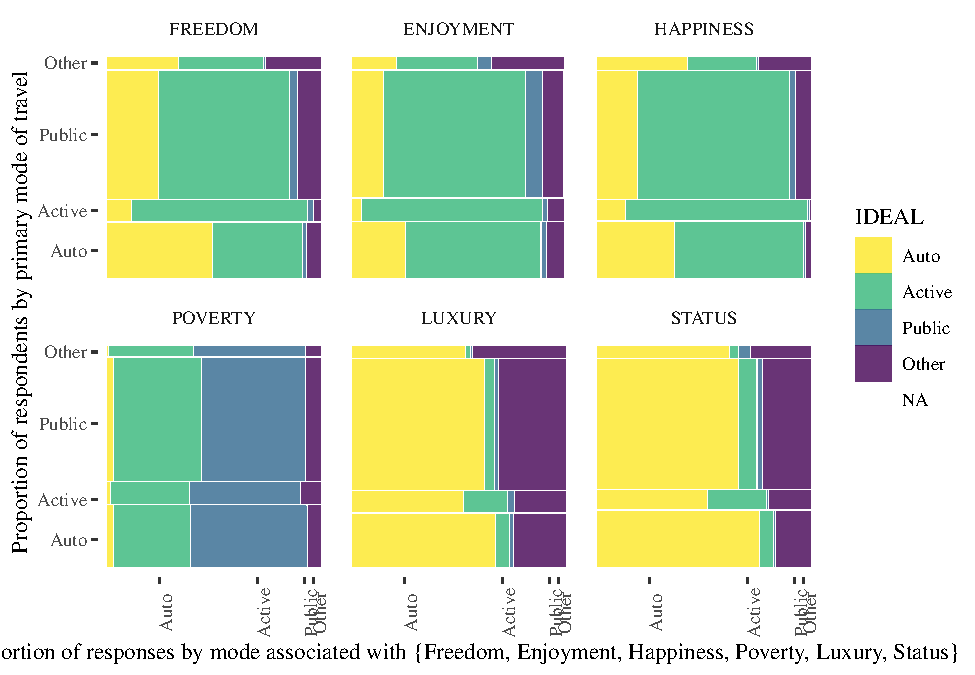
\includegraphics{Dissonance_Santiago_v1_files/figure-latex/figure-mosaic-plots-by-attribute-without-instrumental-1.pdf}
\caption{\label{fig:mosaic-plots-by-attribute}Mosaic plots for affective
values; the y-axis is the proportion of respondents by main mode of
transportation, and the x-axis is the proportion of modes selected for
each value}
\end{figure}

\begin{figure}
\centering
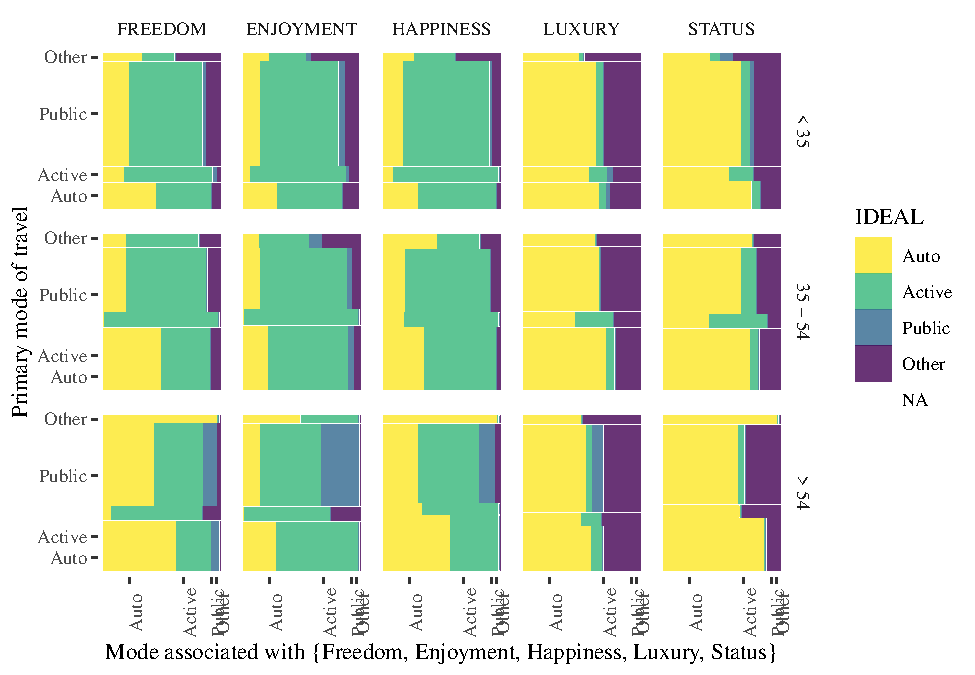
\includegraphics{Dissonance_Santiago_v1_files/figure-latex/figure-mosaic-plots-by-attribute-and-age-without-instrumental-1.pdf}
\caption{\label{fig:mosaic-plots-by-age}Mosaic plots for affective
values by age; the y-axis is the proportion of respondents by main mode
of transportation, and the x-axis is the proportion of modes selected
for each value}
\end{figure}

\begin{figure}
\centering
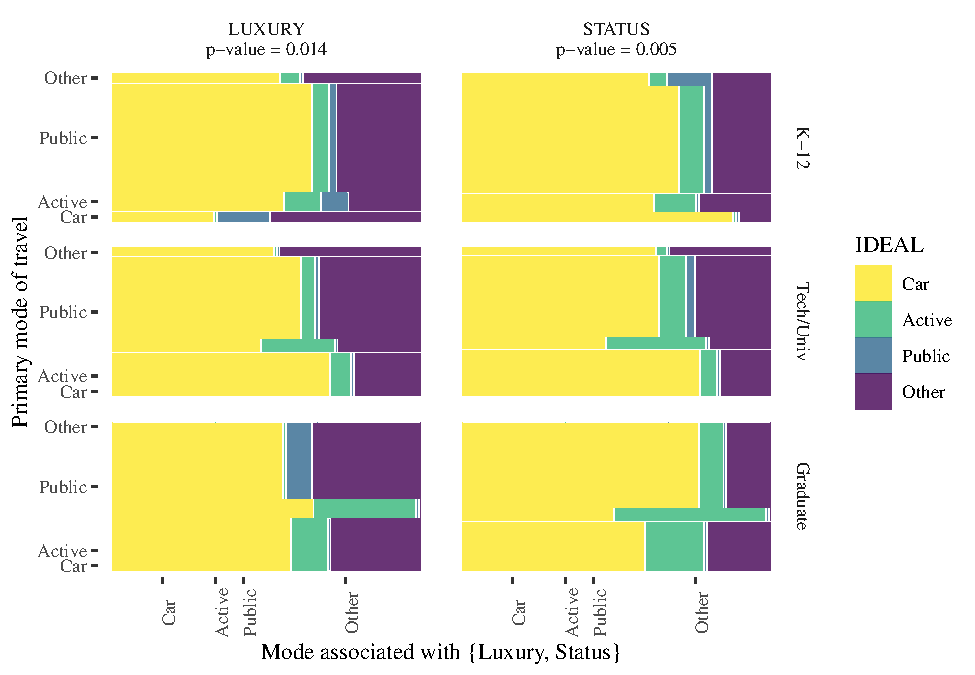
\includegraphics{Dissonance_Santiago_v1_files/figure-latex/figure-mosaic-plots-by-attribute-and-education-without-instrumental-1.pdf}
\caption{\label{fig:mosaic-plots-by-education}Mosaic plots for affective
values by education; the y-axis is the proportion of respondents by main
mode of transportation, and the x-axis is the proportion of modes
selected for each value}
\end{figure}

\begin{figure}
\centering
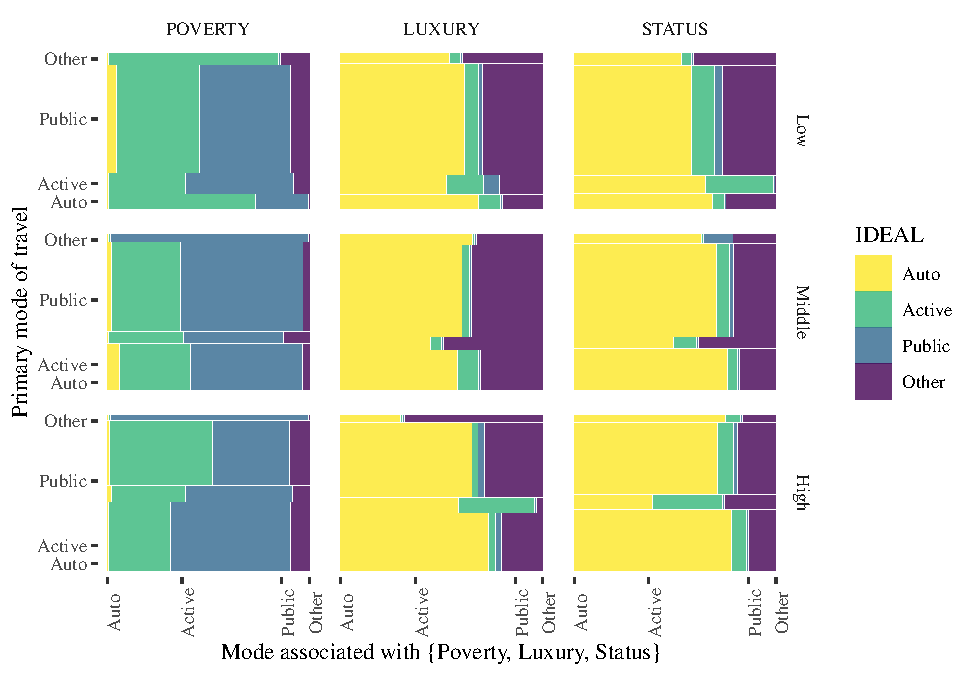
\includegraphics{Dissonance_Santiago_v1_files/figure-latex/figure-mosaic-plots-by-attribute-and-income-without-instrumental-1.pdf}
\caption{\label{fig:mosaic-plots-by-income}Mosaic plots for affective
values by income; the y-axis is the proportion of respondents by main
mode of transportation, and the x-axis is the proportion of modes
selected for each value}
\end{figure}

\begin{figure}
\centering
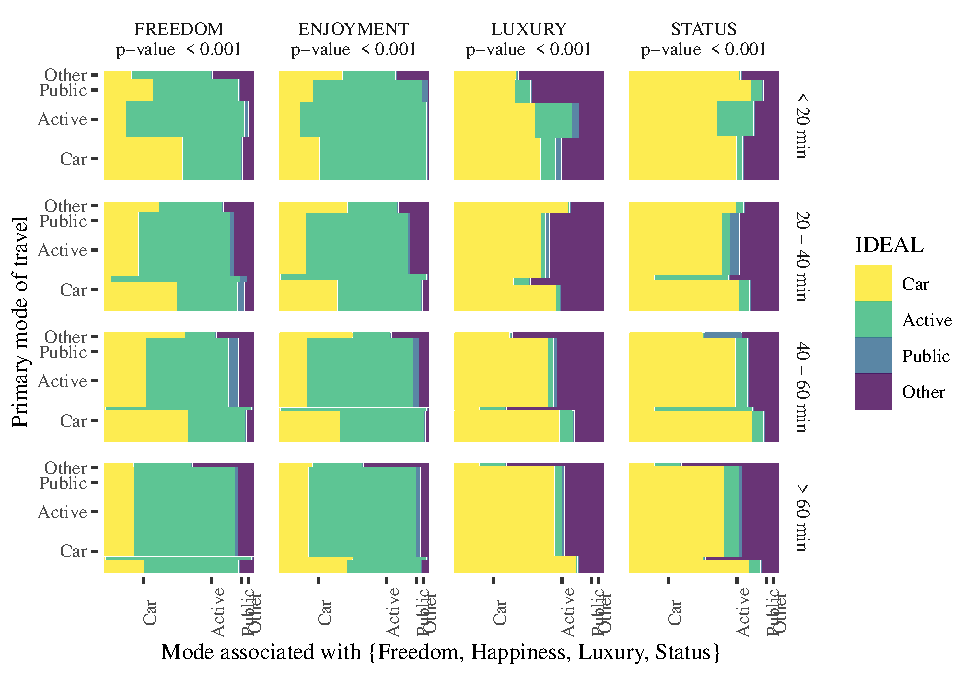
\includegraphics{Dissonance_Santiago_v1_files/figure-latex/figure-mosaic-plots-by-attribute-and-time-without-instrumental-1.pdf}
\caption{\label{fig:mosaic-plots-by-travel-time}Mosaic plots for
affective values by travel time; the y-axis is the proportion of
respondents by main mode of transportation, and the x-axis is the
proportion of modes selected for each value}
\end{figure}

\hypertarget{conclusions}{%
\section{Conclusions}\label{conclusions}}

Words go here.

\hypertarget{references}{%
\section*{References}\label{references}}
\addcontentsline{toc}{section}{References}


\end{document}


